\section{Experimental Evaluation}
\label{sec:results}
% Numerical source: ../data/paper1007.json; no scientific statistics recomputed.
% Display names map existing saved designs; SD unit is stated in each caption.

\newcommand{\HadMainTable}{%
\begin{table*}[!t]
\centering\footnotesize
\setlength{\tabcolsep}{5pt}
\caption{Formal comparison: mean $\pm$ sample SD. Reward $R=-D$ is higher-is-better; friendly-collision mortality $C$ is lower-is-better. Each learned method has three training seeds and 300 common scenes per configuration. Bold marks the best group mean for each metric.}
\label{tab:had-main}
\begin{tabular*}{\textwidth}{@{\extracolsep{\fill}}llrrrr@{}}
\toprule
Method & Metric & ID & $K$-OOD & $N$-OOD & Joint OOD \\
\midrule
\textbf{LEAF} & $R\uparrow$ & $\mathbf{-0.405\pm0.097}$ & $\mathbf{-0.996\pm0.233}$ & $\mathbf{-0.575\pm0.235}$ & $\mathbf{-1.097\pm0.105}$ \\
 & $C\downarrow$ (\%) & $\mathbf{1.33\pm0.45}$ & $\mathbf{1.70\pm0.62}$ & $6.29\pm1.32$ & $4.97\pm1.26$ \\
\addlinespace[2pt]
REFIL & $R\uparrow$ & $-0.715\pm0.049$ & $-1.796\pm0.304$ & $-2.209\pm0.277$ & $-3.308\pm0.303$ \\
 & $C\downarrow$ (\%) & $2.97\pm0.42$ & $4.71\pm0.67$ & $12.86\pm2.14$ & $10.34\pm1.69$ \\
\addlinespace[2pt]
QMIX-Atten & $R\uparrow$ & $-2.318\pm1.431$ & $-5.009\pm2.497$ & $-5.139\pm3.111$ & $-7.415\pm3.970$ \\
 & $C\downarrow$ (\%) & $10.82\pm9.56$ & $12.42\pm9.75$ & $16.38\pm5.43$ & $15.37\pm7.34$ \\
\addlinespace[2pt]
DCG & $R\uparrow$ & $-2.028\pm0.437$ & $-5.839\pm1.920$ & $-5.021\pm2.658$ & $-8.092\pm3.909$ \\
 & $C\downarrow$ (\%) & $9.05\pm3.36$ & $14.97\pm4.68$ & $19.70\pm8.52$ & $19.26\pm10.20$ \\
\addlinespace[2pt]
SPECTra & $R\uparrow$ & $-2.662\pm0.070$ & $-6.933\pm0.670$ & $-6.455\pm1.403$ & $-11.184\pm0.352$ \\
 & $C\downarrow$ (\%) & $13.06\pm0.75$ & $20.71\pm1.60$ & $28.92\pm1.54$ & $31.25\pm1.63$ \\
\addlinespace[2pt]
ALMA & $R\uparrow$ & $-1.326\pm0.193$ & $-3.022\pm0.344$ & $-3.605\pm0.742$ & $-5.375\pm1.036$ \\
 & $C\downarrow$ (\%) & $7.42\pm1.13$ & $9.05\pm1.66$ & $18.42\pm3.84$ & $15.92\pm3.86$ \\
\addlinespace[2pt]
Rule$^{\dagger}$ & $R\uparrow$ & $-1.462\pm0.717$ & $-3.212\pm1.126$ & $-1.545\pm0.881$ & $-3.060\pm0.976$ \\
 & $C\downarrow$ (\%) & $1.98\pm4.47$ & $2.70\pm3.57$ & $\mathbf{5.70\pm3.30}$ & $\mathbf{4.48\pm2.44}$ \\
\bottomrule
\end{tabular*}
\par\vspace{2pt}\parbox{\textwidth}{\footnotesize
$\dagger$ Rule has no training seeds. Its SD is across the 300 scene seeds, after averaging configurations within each scene. All other SDs measure training-seed variation. Collision SDs are percentage points.}
\end{table*}}

\newcommand{\HadCoreAblationTable}{%
\begin{table*}[!t]
\centering\footnotesize
\setlength{\tabcolsep}{5pt}
\caption{Trained design comparisons: absolute reward $R=-D$ and friendly-collision mortality $C$, mean $\pm$ sample SD across three training seeds. Each configuration uses 300 common scenes. Bold marks the best mean among these five designs.}
\label{tab:had-core-ablation}
\begin{tabular*}{\textwidth}{@{\extracolsep{\fill}}llrrrr@{}}
\toprule
Method & Metric & ID & $K$-OOD & $N$-OOD & Joint OOD \\
\midrule
\textbf{LEAF} & $R\uparrow$ & $\mathbf{-0.405\pm0.097}$ & $\mathbf{-0.996\pm0.233}$ & $\mathbf{-0.575\pm0.235}$ & $\mathbf{-1.097\pm0.105}$ \\
 & $C\downarrow$ (\%) & $\mathbf{1.33\pm0.45}$ & $\mathbf{1.70\pm0.62}$ & $\mathbf{6.29\pm1.32}$ & $\mathbf{4.97\pm1.26}$ \\
\addlinespace[2pt]
Memory query & $R\uparrow$ & $-0.527\pm0.227$ & $-1.529\pm0.734$ & $-0.998\pm0.621$ & $-1.946\pm1.229$ \\
 & $C\downarrow$ (\%) & $1.66\pm0.86$ & $2.59\pm1.78$ & $8.57\pm4.41$ & $6.65\pm4.16$ \\
\addlinespace[2pt]
No host & $R\uparrow$ & $-0.510\pm0.138$ & $-1.768\pm0.621$ & $-1.263\pm0.653$ & $-2.319\pm0.889$ \\
 & $C\downarrow$ (\%) & $2.23\pm0.77$ & $3.67\pm1.65$ & $10.71\pm3.98$ & $8.76\pm3.14$ \\
\addlinespace[2pt]
Direct read & $R\uparrow$ & $-0.928\pm0.210$ & $-1.958\pm0.457$ & $-2.020\pm0.446$ & $-3.196\pm0.687$ \\
 & $C\downarrow$ (\%) & $3.34\pm1.66$ & $4.46\pm2.10$ & $11.16\pm1.81$ & $9.17\pm2.18$ \\
\addlinespace[2pt]
One round & $R\uparrow$ & $-0.609\pm0.272$ & $-1.203\pm0.402$ & $-1.355\pm0.884$ & $-2.157\pm1.006$ \\
 & $C\downarrow$ (\%) & $1.57\pm0.15$ & $2.08\pm0.32$ & $8.35\pm3.16$ & $6.56\pm2.37$ \\
\bottomrule
\end{tabular*}
\par\vspace{2pt}\parbox{\textwidth}{\footnotesize
Configurations are weighted equally within each training seed. Memory query adds incoming GRU history to LEAF's reader query. No host removes the local host, imagination, and associated losses from the memory-query design. Direct read and One round retain query history and execute zero and one contextual update, respectively. Collision SDs are percentage points.}
\end{table*}}

\newcommand{\HadFullVariantTable}{%
\begin{table*}[!t]
\centering\footnotesize
\setlength{\tabcolsep}{5pt}
\caption{All ten completed trained designs: reward mean $\pm$ sample SD across three training seeds on the same formal matrix. Bold marks the best group mean. All designs share the evaluation configurations.}
\label{tab:had-full-variants}
\begin{tabular*}{\textwidth}{@{\extracolsep{\fill}}lrrrr@{}}
\toprule
Method & ID & $K$-OOD & $N$-OOD & Joint OOD \\
\midrule
\textbf{LEAF} & $\mathbf{-0.405\pm0.097}$ & $\mathbf{-0.996\pm0.233}$ & $-0.575\pm0.235$ & $\mathbf{-1.097\pm0.105}$ \\
Memory query & $-0.527\pm0.227$ & $-1.529\pm0.734$ & $-0.998\pm0.621$ & $-1.946\pm1.229$ \\
No host & $-0.510\pm0.138$ & $-1.768\pm0.621$ & $-1.263\pm0.653$ & $-2.319\pm0.889$ \\
Direct read & $-0.928\pm0.210$ & $-1.958\pm0.457$ & $-2.020\pm0.446$ & $-3.196\pm0.687$ \\
One round & $-0.609\pm0.272$ & $-1.203\pm0.402$ & $-1.355\pm0.884$ & $-2.157\pm1.006$ \\
Last read & $-0.434\pm0.083$ & $-1.020\pm0.100$ & $-0.652\pm0.160$ & $-1.269\pm0.202$ \\
Fixed depth & $-0.407\pm0.204$ & $-1.004\pm0.665$ & $-0.659\pm0.184$ & $-1.265\pm0.230$ \\
Initial keys & $-0.469\pm0.091$ & $-1.221\pm0.344$ & $-1.778\pm1.292$ & $-2.370\pm1.164$ \\
Unshared rounds & $-0.476\pm0.183$ & $-1.127\pm0.157$ & $\mathbf{-0.543\pm0.156}$ & $-1.232\pm0.253$ \\
Count inputs & $-0.596\pm0.145$ & $-1.301\pm0.427$ & $-1.075\pm0.449$ & $-1.685\pm0.844$ \\
\bottomrule
\end{tabular*}
\par\vspace{2pt}\parbox{\textwidth}{\footnotesize
The five core names follow Table~\ref{tab:had-core-ablation}. Last read uses only the final read; Fixed depth trains and executes four rounds; Initial keys anchors keys and values to the initial entity set; Unshared rounds trains four independent update blocks; Count inputs adds typed-count features. These five designs also retain query history. Unshared rounds is compared with Fixed depth to separate sharing under a matched depth schedule.}
\end{table*}}

\newcommand{\HadCapacityTable}{%
\begin{table*}[!t]
\centering\footnotesize
\setlength{\tabcolsep}{5pt}
\caption{Capacity reference: reward and friendly-collision mortality, mean $\pm$ sample SD across three training seeds. The enlarged REFIL reference approximately matches LEAF's actor parameter budget; all methods use the same formal evaluation scenes.}
\label{tab:had-capacity}
\begin{tabular*}{\textwidth}{@{\extracolsep{\fill}}llrrrr@{}}
\toprule
Method & Metric & ID & $K$-OOD & $N$-OOD & Joint OOD \\
\midrule
\textbf{LEAF} & $R\uparrow$ & $\mathbf{-0.405\pm0.097}$ & $\mathbf{-0.996\pm0.233}$ & $\mathbf{-0.575\pm0.235}$ & $\mathbf{-1.097\pm0.105}$ \\
 & $C\downarrow$ (\%) & $\mathbf{1.33\pm0.45}$ & $\mathbf{1.70\pm0.62}$ & $\mathbf{6.29\pm1.32}$ & $\mathbf{4.97\pm1.26}$ \\
\addlinespace[2pt]
REFIL & $R\uparrow$ & $-0.715\pm0.049$ & $-1.796\pm0.304$ & $-2.209\pm0.277$ & $-3.308\pm0.303$ \\
 & $C\downarrow$ (\%) & $2.97\pm0.42$ & $4.71\pm0.67$ & $12.86\pm2.14$ & $10.34\pm1.69$ \\
\addlinespace[2pt]
REFIL (matched) & $R\uparrow$ & $-0.914\pm0.165$ & $-2.493\pm0.280$ & $-2.269\pm0.312$ & $-4.170\pm0.760$ \\
 & $C\downarrow$ (\%) & $4.12\pm0.46$ & $6.86\pm2.30$ & $12.40\pm3.09$ & $12.02\pm4.17$ \\
\bottomrule
\end{tabular*}
\par\vspace{2pt}\parbox{\textwidth}{\footnotesize
Actor parameter counts are 175,754 for LEAF, 102,025 for REFIL, and 176,393 for REFIL (matched). Collision SDs are percentage points.}
\end{table*}}


\noindent\textbf{Setup.}
We evaluate target protection in the planar model of SkyHAD 3.0.0~\cite{skyhad2026}, with public entity-state observations, a fixed reactive--rush attacker, and a horizon of 100 physical steps. Training samples balanced teams $N_R=N_B=N\in\{4,6,8,10\}$ and target counts $K\in\{1,2,3\}$. Each learned method uses three training seeds and a budget of $10^6$ physical environment steps per seed. LEAF has hidden width 64, four attention heads, learning rate $5\times10^{-4}$, discount 0.99, batch size 32, and replay capacity 5000. Training samples one to four relational rounds; formal evaluation uses four.

Final policies execute with frozen parameters on 24 configurations, each with 300 common initial scenes. In-distribution (ID) configurations are $(4,4,2)$, $(6,6,2)$, $(8,8,2)$, and $(10,10,3)$, written as $(N_R,N_B,K)$. Target-count extrapolation ($K$-OOD) uses $(10,10,K)$ for $K\in\{4,6,9,12\}$; team-size extrapolation ($N$-OOD) uses $(N,N,2)$ for $N\in\{15,20,25,30,40,50\}$. Joint extrapolation combines $N\in\{15,20,30\}$ with $K\in\{4,6\}$ and includes $(30,30,9)$ and $(30,30,12)$. The remaining configurations, $(5,5,2)$ and $(10,10,2)$, provide intermediate-scale reference points. The five learned baselines are REFIL~\cite{iqbal2021refil}, QMIX with an entity-attention encoder (QMIX-Atten)~\cite{rashid2018qmix}, DCG~\cite{boehmer2020dcg}, SPECTra~\cite{park2026spectra}, and ALMA~\cite{iqbal2022alma}. Rule provides a fixed-controller reference.

\noindent\textbf{Metrics and aggregation.}
The primary metric is episode reward $R=-D$, with higher values indicating better target protection. Friendly-collision mortality,
\begin{equation}
 C=\frac{\text{defenders killed by friendly collision}}{N_R},
\end{equation}
measures losses within the protecting team. Each model first averages the 300 scenes within a configuration and then averages configurations equally within a group. Tables report mean $\pm$ sample standard deviation (SD) across the three trained models~\cite{agarwal2021rliable}. For Rule, the reported SD is across 300 scene seeds after averaging configurations within each seed.

Learning curves use 50 validation checkpoints. Each checkpoint evaluates four ID configurations with 25 fixed scenes each, separate from the formal evaluation scenes. We align validation indices across training seeds and plot the mean reward at the mean recorded environment-step count. Bands show the three-model sample SD, without smoothing.

\subsection{Comparison Across Deployment Populations}
\label{subsec:comparison}
LEAF obtains the highest group mean reward among the six learned methods and Rule in all four groups (Table~\ref{tab:had-main}). Relative to REFIL, the reward gains are 0.310, 0.800, 1.635, and 2.211 for ID, $K$-OOD, $N$-OOD, and Joint OOD, respectively. All three corresponding training-seed comparisons favor LEAF in each group. The larger gains under team-size and joint extrapolation show the value of the relational encoder when a defender must coordinate within a larger entity set.

Figure~\ref{fig:had-generalization} connects learning to deployment. At the tenth validation checkpoint, approximately $0.2$ million environment steps, LEAF reaches $-2.046\pm0.028$ compared with REFIL's $-4.429\pm0.284$. At the final checkpoint, the rewards are $-0.373\pm0.066$ and $-0.738\pm0.122$. The other panels follow the frozen policies as target count, team size, and both populations increase. Presenting each joint configuration separately preserves the distinct changes in threats and assets.

LEAF also has lower mean friendly-collision mortality than each learned baseline in all four groups. Rule incurs fewer collision deaths in $N$-OOD and Joint OOD, at 5.70\% and 4.48\%, compared with LEAF's 6.29\% and 4.97\%. Its corresponding rewards are lower. The two metrics therefore distinguish conserving defenders from protecting the targets: LEAF combines low friendly losses with more effective defense.

\HadMainTable

\begin{figure*}[!t]
\centering
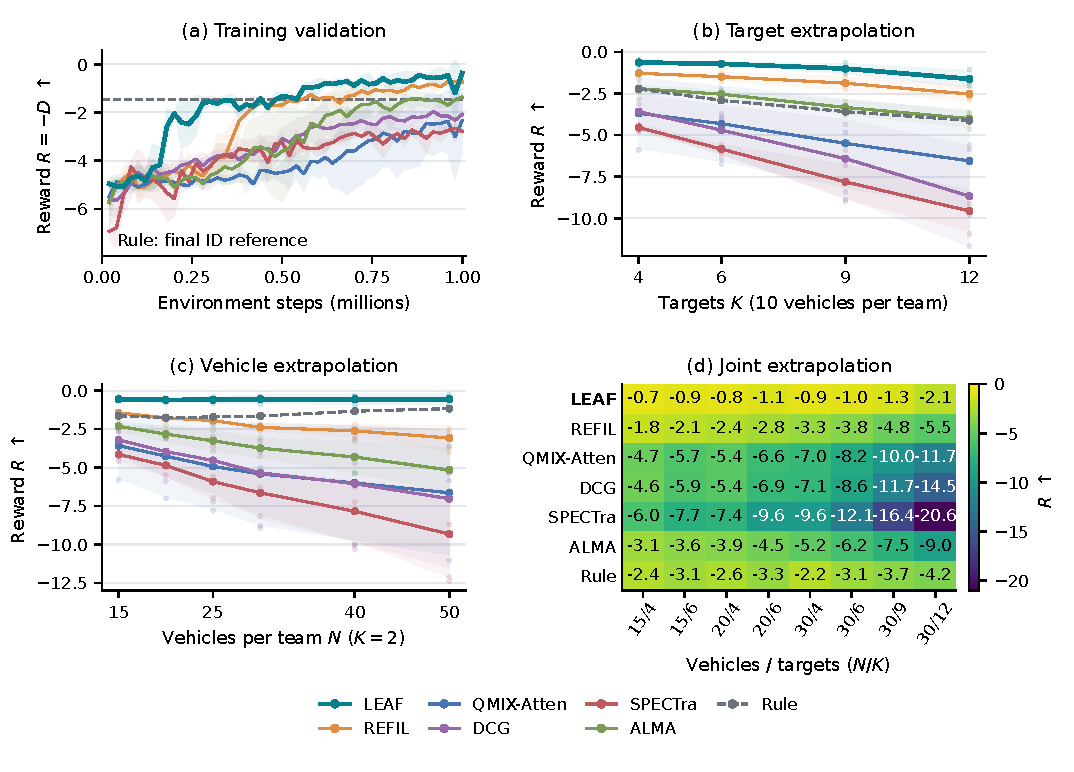
\includegraphics[width=\textwidth]{figures/fig_had_generalization.pdf}
\caption{Learning and population transfer. (a) Fifty validation checkpoints for LEAF and five learned baselines at recorded environment steps; bands show one model-seed sample SD. The Rule line marks its final ID reward. (b)--(c) Frozen-policy reward under target-count and team-size extrapolation, with seed points and SD bands for learned methods. (d) Reward at the eight joint-extrapolation configurations on a common linear scale.}
\label{fig:had-generalization}
\end{figure*}

\subsection{Ablation and Design Comparisons}
\label{subsec:ablation}
The trained comparisons address three aspects of the encoder: constructing context before reading, locating temporal memory, and combining the relational feature with its host. Table~\ref{tab:had-core-ablation} and Fig.~\ref{fig:had-ablation} give both learning trajectories and population-transfer results. The \emph{Memory query} design adds detached previous GRU state to the reader query. \emph{Direct read}, \emph{One round}, and \emph{No host} use this same memory-query formulation, providing the paired design comparisons below.

\noindent\textbf{Context before reading.}
Direct read applies the reader to the initial entity representations. One round performs one shared contextual update before reading. The latter improves group mean reward by 0.319, 0.755, 0.665, and 1.039 in ID, $K$-OOD, $N$-OOD, and Joint OOD, with two of three seed pairs improving in each group. The consistent direction across population groups supports processing entity relationships before compressing them into the defender's decision feature.

\noindent\textbf{Current-state reading with downstream memory.}
Memory query and LEAF both preserve the recurrent decision network. Using only the current self state for the query gives LEAF mean reward gains of 0.122, 0.533, 0.424, and 0.849 across the four groups. The gains hold for three seeds in ID and two seeds in each extrapolation group. The result favors the chosen division of computation: the reader extracts the current relational context, and the downstream GRU combines it with temporal history.

\noindent\textbf{Integration with cooperative value learning.}
No host retains the relational path while removing the REFIL feature path, imagined branches, and associated auxiliary loss. Restoring this host in the Memory query design improves the three extrapolation-group rewards by 0.239, 0.265, and 0.372; the ID mean changes by $-0.017$. LEAF then combines the retained host with current-state reading. Although No host reaches a final ID validation reward of $-0.381\pm0.126$, close to LEAF's $-0.373\pm0.066$, their transfer results differ substantially. This contrast shows why the evaluation must examine deployment populations alongside training validation.

\HadCoreAblationTable

\begin{figure*}[!t]
\centering
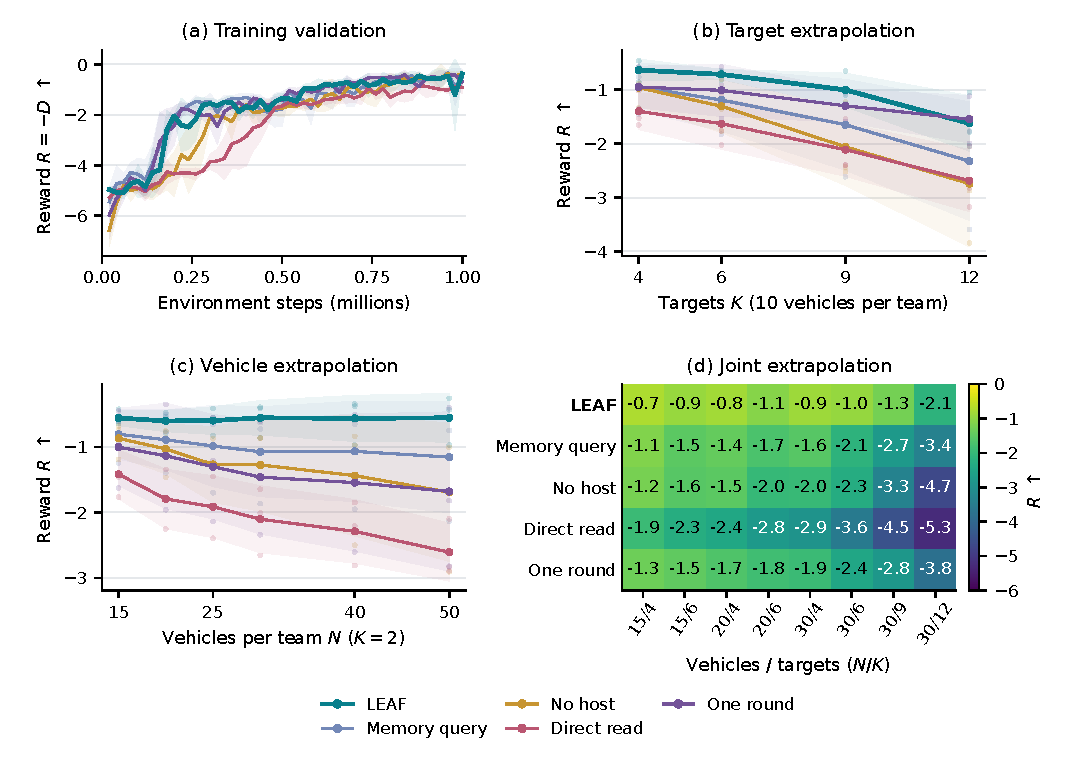
\includegraphics[width=\textwidth]{figures/fig_had_ablation.pdf}
\caption{Trained design comparisons. (a) Validation reward over 50 checkpoints; lines and bands show the three-model mean and sample SD at actual mean environment steps. (b)--(c) Target-count and team-size extrapolation. (d) Joint-extrapolation rewards on a common linear scale. Memory query adds temporal state to LEAF's reader. Direct read, One round, and No host use that memory-query formulation; their paired comparisons are described in the text.}
\label{fig:had-ablation}
\end{figure*}

A parameter-matched REFIL control has 176,393 actor parameters, close to LEAF's 175,754; standard REFIL has 102,025. Its group rewards are $-0.914\pm0.165$, $-2.493\pm0.280$, $-2.269\pm0.312$, and $-4.170\pm0.760$. LEAF exceeds this control in all three seed comparisons for every group. The performance gain thus persists when the host is given a comparable parameter budget.

\subsection{Mechanism of Relational Encoding}
\label{subsec:mechanism}
The mechanism study follows the computation introduced in Section~\ref{sec:method}: contextual updates produce intermediate entity sets, the self-conditioned reader combines them into a decision feature, and the resulting actions determine interception and protection. We examine execution at the depths used during training, record the normal intermediate reads, and relate the policy's outcome to the formal protection metrics.

\noindent\textbf{Protection across processing depths.}
We execute each frozen LEAF model at $L\in\{1,2,3,4\}$ on ten common scenes in each of three configurations: $(10,10,2)$, $(30,30,2)$, and $(30,30,12)$. The first two vary team size at fixed target count; the last two vary target count at fixed team size. All four paths use the trained update block, reader, fusion, and recurrent decision network. REFIL runs on the same scenes. Reward is averaged over scenes within each model and then reported across three model seeds; differences between depths are paired by model and scene.

Figure~\ref{fig:leaf-depth} shows that all four LEAF depths have higher mean reward than REFIL in these three configurations. At 10v10 and 30v30 with two targets, two-round execution has paired reward differences of $-0.273\pm0.047$ and $-0.363\pm0.291$ relative to four rounds, with all three model means lower. Three and four rounds give the same reward at 10v10; three rounds give $0.146\pm0.131$ higher reward at 30v30 with two targets and $0.793\pm0.907$ lower reward with twelve targets. Thus the ordering of execution depths changes with the engagement. Together with the trained Direct read--One round comparison, these results locate the common advantage in useful contextual representations, with later processing altering protection according to the scene.

\begin{figure*}[!t]
\centering
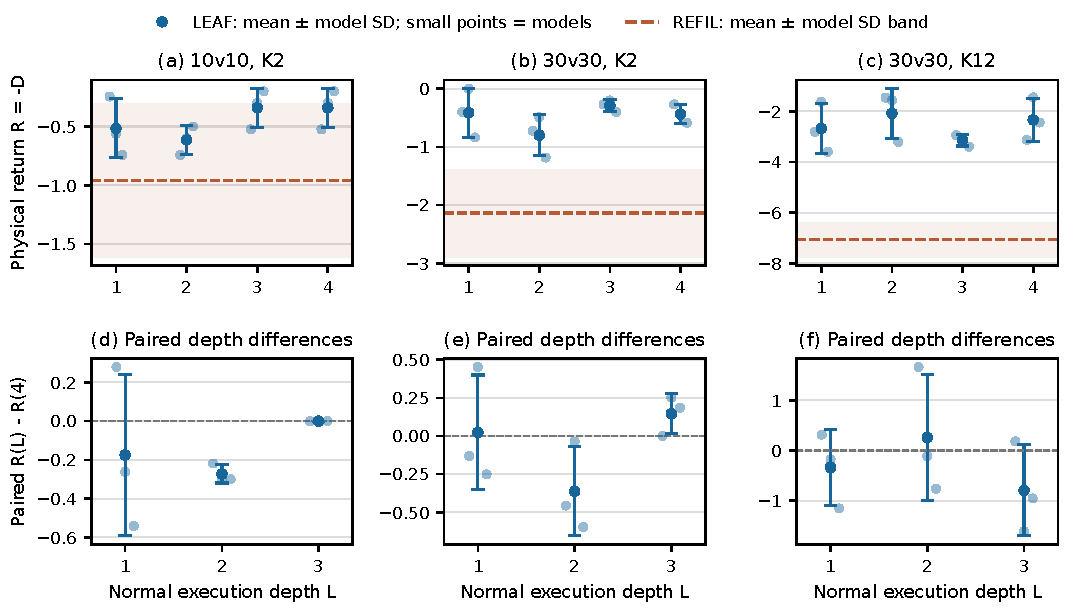
\includegraphics[width=\textwidth]{figures/fig_leaf_depth.pdf}
\caption{Frozen LEAF execution at depths used during training. Top: reward at each depth and the REFIL reference. Bottom: scene-paired reward difference from four-round execution; positive values favor the shorter path. Each point and error bar is the mean and sample SD of three model means, each based on ten scenes. Small points show individual models.}
\label{fig:leaf-depth}
\end{figure*}

\noindent\textbf{Intermediate reading varies with the defender and time.}
We record all four read vectors and fusion weights during the normal four-round executions: 90 episodes containing 38,693 live-defender decisions. Figure~\ref{fig:leaf-readout}(a) shows a clear preference for early context. The first read receives 73.66--75.65\% of mean fusion weight across the three configurations, and the first two together receive approximately 99\%. The encoder therefore supplies its recurrent policy primarily with the early contextual reads even when it executes all four updates.

The same average preference encompasses different choices by individual defenders. For the first-round weight, the within-state SD across active defenders averages 11.44, 13.91, and 12.68 percentage points in the three configurations. Tracking the same defender across adjacent physical steps gives mean absolute weight changes of 5.49, 5.34, and 5.36 percentage points. These measurements directly characterize the self-conditioned fusion: defenders observing the same engagement combine stages differently, and each defender changes that combination as the engagement evolves. The shared encoder consequently offers a common relational computation with receiver-specific access to its intermediate stages.

\begin{figure*}[!t]
\centering
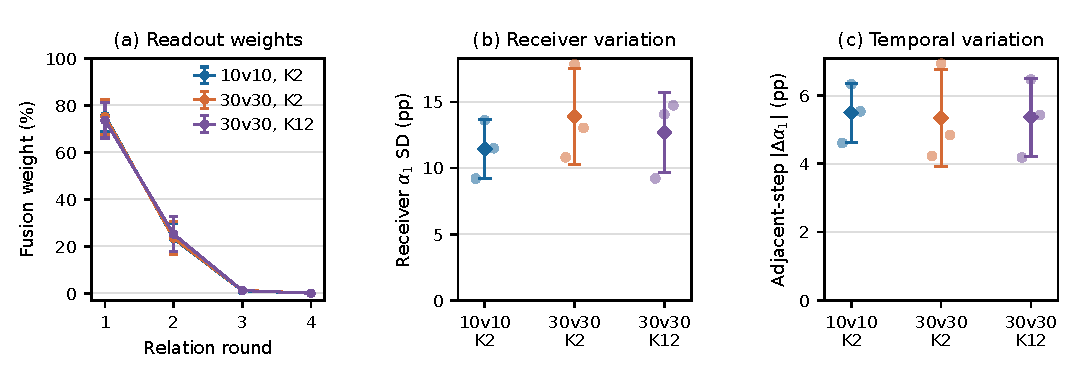
\includegraphics[width=\textwidth]{figures/fig_leaf_readout.pdf}
\caption{Intermediate-read use in normal four-round execution. (a) Mean fusion weights by round and configuration. (b) Variation among active defenders at the same physical step, measured by the population SD of the first-round weight. (c) Mean absolute change of that weight for the same defender at adjacent physical steps. Panel (b) averages over physical decision states within each model. Panel (c) averages the adjacent-step changes within each episode and then weights the ten scenes equally. Error bars show sample SD across three model means; small points retain the models in (b)--(c).}
\label{fig:leaf-readout}
\end{figure*}

\noindent\textbf{From coordinated response to target protection.}
The formal evaluation uses 300 scenes per model and configuration. Across the three mechanism configurations and the larger 50v50 case, LEAF combines higher attacker interception with lower friendly-collision mortality and less frequent target damage than REFIL. At 10v10 with two targets, interception increases from 77.00\% to 86.38\%, and target-damage incidence falls from 55.22\% to 30.44\%. At 30v30 with two targets, interception rises from 75.11\% to 83.02\% and target-damage incidence falls from 70.89\% to 29.56\%. Increasing the targets from two to twelve at the same team size preserves this direction: LEAF intercepts 81.54\% of attackers and experiences target damage in 48.33\% of episodes, compared with 74.48\% and 78.22\% for REFIL. At 50v50, LEAF retains an interception advantage of 6.41 percentage points and reduces friendly-collision mortality from 19.59\% to 11.14\%; target-damage incidence falls from 70.56\% to 28.11\%. The learned representation thus supports the intended team outcome: fewer defenders are lost to one another, more threats are intercepted, and fewer episodes allow damage to the protected assets.





\begin{figure*}[!t]
\centering
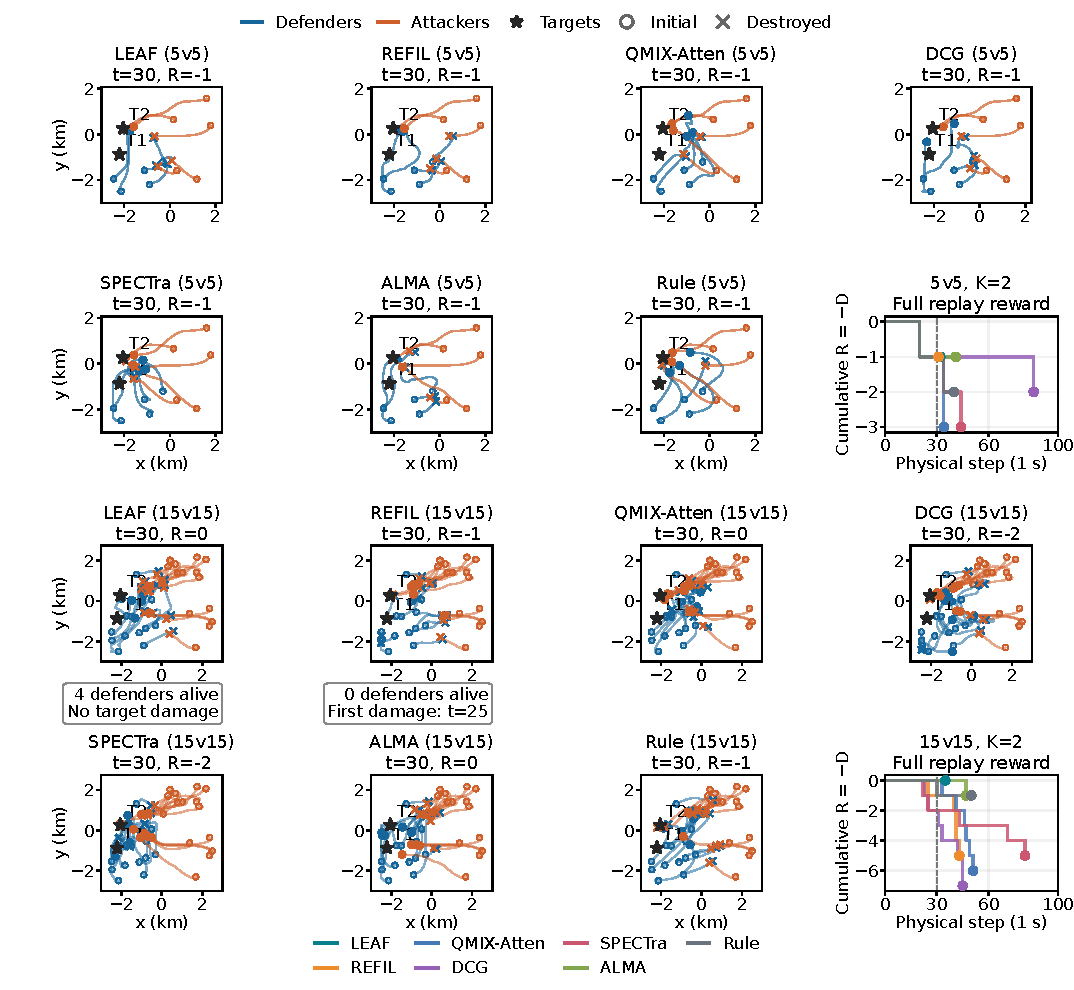
\includegraphics[width=\textwidth]{figures/fig_leaf_final1007_trajectory.pdf}
\caption{Common-scene trajectory comparison. The upper two rows show 5v5 and the lower two show 15v15, both with two targets. Each block contains seven spatial panels and a cumulative-reward plot. Paths end at the common snapshot step 30: open circles are initial positions, filled circles are live vehicles, crosses are destroyed vehicles, and stars are targets. Panel titles give reward at the snapshot. Reward curves end at the actual terminal step, marked by a dot; the dashed line marks the snapshot time. The annotations identify the two methods' defensive state at step 30 in the 15v15 case. All spatial panels within a scale share coordinates and color conventions.}
\label{fig:had-cases}
\end{figure*}

\subsection{Representative Trajectories}
\label{subsec:trajectories}
Figure~\ref{fig:had-cases} compares all seven methods at $(5,5,2)$ and $(15,15,2)$ under the same initial layout within each configuration. Learned policies use training seed 0, and both examples use scene seed 9000. Paths and entity states are shown at physical step 30; the adjacent reward curves continue to each policy's actual terminal step.

At 5v5, LEAF, REFIL, and ALMA finish with reward $-1$. LEAF and REFIL first incur target damage at step 20 and complete their engagements at steps 32 and 31. Their trajectories show different interception routes with the same final protection outcome.

The 15v15 scene exposes the effect of sustaining the defense. At the common snapshot, LEAF retains four defenders against two surviving attackers, with both targets undamaged. REFIL has lost its final defender at step 27; four attackers remain at step 30, and reward has reached $-1$. Its reward then falls to $-5$ as damage continues after the defending team disappears. LEAF intercepts all 15 attackers by step 35 and finishes with $R=0$. QMIX-Atten, DCG, SPECTra, ALMA, and Rule finish with $-6$, $-7$, $-5$, $-1$, and $-1$, respectively. The surviving-team snapshots and complete reward histories connect maintained defensive capability to the final protection outcome.


